\documentclass[11pt]{article}

\usepackage[margin=0.75in]{geometry}
\usepackage[T1]{fontenc}
\usepackage[utf8]{inputenc}
\usepackage{lmodern}
\usepackage{microtype}
\usepackage{booktabs}
\usepackage{tabularx}
\usepackage{longtable}
\usepackage{array}
\usepackage{enumitem}
\usepackage{caption}
\usepackage{float}
\usepackage{xcolor}
\usepackage{seqsplit}
\usepackage{amsmath}
\usepackage{tikz}
\usepackage{pgfplots}
\usepackage{pdflscape}
\usepackage{hyperref}
\usetikzlibrary{arrows.meta, positioning, calc}
\pgfplotsset{compat=1.18}

\hypersetup{
  colorlinks=true,
  linkcolor=black,
  urlcolor=blue!55!black,
  citecolor=black
}

\definecolor{BoxBlue}{RGB}{226,236,248}
\definecolor{BoxGreen}{RGB}{226,241,232}
\definecolor{BoxYellow}{RGB}{250,242,220}
\definecolor{BoxRed}{RGB}{248,226,226}
\definecolor{LineGray}{RGB}{90,90,90}
\definecolor{BarBlue}{RGB}{78,121,167}
\definecolor{BarGreen}{RGB}{89,161,79}
\definecolor{BarOrange}{RGB}{242,142,44}

\newcommand{\id}[1]{\texttt{\expandafter\seqsplit\expandafter{\detokenize{#1}}}}
\newcommand{\bigO}{\mathcal{O}}
\newcolumntype{Y}{>{\raggedright\arraybackslash}X}
\newcolumntype{L}[1]{>{\raggedright\arraybackslash}p{#1}}
\setlist[itemize]{leftmargin=1.25em, itemsep=0.25em}
\setlist[enumerate]{leftmargin=1.45em, itemsep=0.25em}
\captionsetup{font=small, labelfont=bf}

\title{\textbf{V2 Search Benchmark Work Review}\\
\large Algorithm 4, Failure Learning, DrugEye Benchmarking, and Complexity}
\author{medicine-search-clean}
\date{Engineering briefing}

\begin{document}
\maketitle

\begin{abstract}
This document summarizes the V2 search work completed today. It is written for
an engineering review: plain language first, then implementation details,
complexity analysis, benchmark results, category-level error rates, and concrete
examples. The central point is that the work did not add manual lookup answers.
The hardcoded alias path was removed, the failures were converted into general
ranking and candidate-generation rules, and the benchmark was rerun on the
manual set, a 6,000-row proportional sample, and the full 115,000-row V2
dataset.
\end{abstract}

\section{Plain-Language Summary}

Think of the search system as a pharmacist assistant. A user may type a medicine
name with missing letters, wrong vowels, a keyboard slip, OCR mistakes, or extra
strength words like \id{500mg}. The assistant should find the right family, but
it should also know when the input is dangerous and should not confidently pick
one product.

Today we did four main things:

\begin{enumerate}
  \item Cleaned the Algorithm 4 story after discovering that manual aliases
        would be cheating. The final code has no hardcoded manual-case mapping.
  \item Turned the supplied mistake analysis into general rules: first-letter
        variants, stronger tie breakers, prefix-only penalties, and broader
        confusion-pair handling.
  \item Reran Algorithm 4 on the manual 50 cases, the 6,000-row proportional
        sample, and the full V2 dataset.
  \item Documented time and space complexity for all algorithms and benchmarked
        DrugEye on the same 6,000-row sample for external comparison.
\end{enumerate}

The result is useful but not magic. Algorithm 4 is safer than Algorithm 2 and
better than Algorithm 1/2 on full V2 aggregate scores. It slightly beats
Algorithm 3 on Hit@1, but after the broader recommendation pass it trails
Algorithm 3 on Hit@20 and behavior success. So Algorithm 3 remains the cleaner
production baseline; Algorithm 4 is a serious optimization/research direction,
not a final replacement.

\section{What Changed Today}

\begin{table}[H]
\centering
\small
\begin{tabularx}{\linewidth}{L{0.21\linewidth}Y L{0.25\linewidth}}
\toprule
\textbf{Work item} & \textbf{What changed} & \textbf{Evidence} \\
\midrule
Removed cheating path &
The manual alias table and alias rescue path were removed from Algorithm 4. &
\id{rg} found no alias mapping path in Algorithm 4. \\
Learned from supplied mistakes &
Added general first-letter variants, same-position/length tie breakers,
expanded \id{M/N} confusion, and prefix-only penalties. &
\path{benchmark_01_legacy/master_algorithms/algorithm_4_commercial_name_search.py} \\
Manual rerun &
Reran the 50 manually supplied failed cases after the recommendation pass. &
Hit@1 58.00\%, Hit@20 70.00\%, unsafe 0.00\%. \\
Sample rerun &
Reran Algorithm 4 on the deterministic 6,000-row proportional sample. &
Hit@1 81.12\%, Hit@20 92.83\%, unsafe 0.00\%. \\
Full rerun &
Reran Algorithm 4 on all 115,000 V2 cases. &
Hit@1 81.86\%, Hit@20 92.99\%, behavior 93.09\%. \\
DrugEye benchmark &
Benchmarked the public DrugEye trade-name path on the same 6,000-row sample. &
Hit@1 21.75\%, Hit@20 30.53\%, no-result 62.88\%. \\
Documentation &
Updated README, Algorithm 4 design, manual failure analysis, and complexity notes. &
\path{benchmark_02_synthetic/docs/} \\
\bottomrule
\end{tabularx}
\caption{Work completed in today's V2 review session.}
\end{table}

\section{Algorithms Compared}

\begin{table}[H]
\centering
\small
\begin{tabularx}{\linewidth}{L{0.16\linewidth}L{0.30\linewidth}Y}
\toprule
\textbf{Label} & \textbf{Implementation} & \textbf{Role in the benchmark} \\
\midrule
Algorithm 1 & Current app evaluator & Conservative existing app behavior, large candidate pool, good safety behavior. \\
Algorithm 2 & External English fast algorithm & Strong typo retrieval, but unsafe confident top-1 behavior was high. \\
Algorithm 3 & Master rank-fusion algorithm & Runs Algorithm 1 and Algorithm 2, fuses them, then applies safety gates. \\
Algorithm 4 & Algorithm 2 plus family rescue/safety layer & Avoids Algorithm 1's full query path, adds bounded family rescue and clarification gates. \\
DrugEye trade & Public DrugEye website trade-name search & External website baseline, sampled because it is a public serial website call. \\
\bottomrule
\end{tabularx}
\caption{Human-facing algorithm names used in the V2 reports.}
\end{table}

\section{One Worked Example}

\subsection*{Input: \id{flacton}}

This is a useful example because it shows both progress and the remaining
problem.

\begin{table}[H]
\centering
\small
\begin{tabularx}{\linewidth}{L{0.25\linewidth}Y}
\toprule
\textbf{Field} & \textbf{Value} \\
\midrule
Input & \id{flacton} \\
Expected family & \id{FLECTOR} \\
Manual-set pattern & multi-substitution \\
Old Algorithm 1/2/3 rank & not found within top 20 \\
Latest Algorithm 4 rank & 2 \\
Latest top 5 & \id{FLU CUT N}, \id{FLECTOR}, \id{FRACTIN}, \id{FLATICON}, \id{SLAFTON} \\
Safety result & ambiguous, not confident \\
\bottomrule
\end{tabularx}
\caption{The concrete example used for the step-by-step explanation.}
\end{table}

Plainly: before today's recommendation pass, all first three algorithms missed
\id{FLECTOR} within the top 20 for \id{flacton}. After the general rescue
changes, Algorithm 4 finds \id{FLECTOR} at rank 2. It still has a wrong top-1
neighbor, so the safety gate is important: the system must show candidates and
avoid confident dispensing.

\begin{figure}[H]
\centering
\resizebox{\linewidth}{!}{%
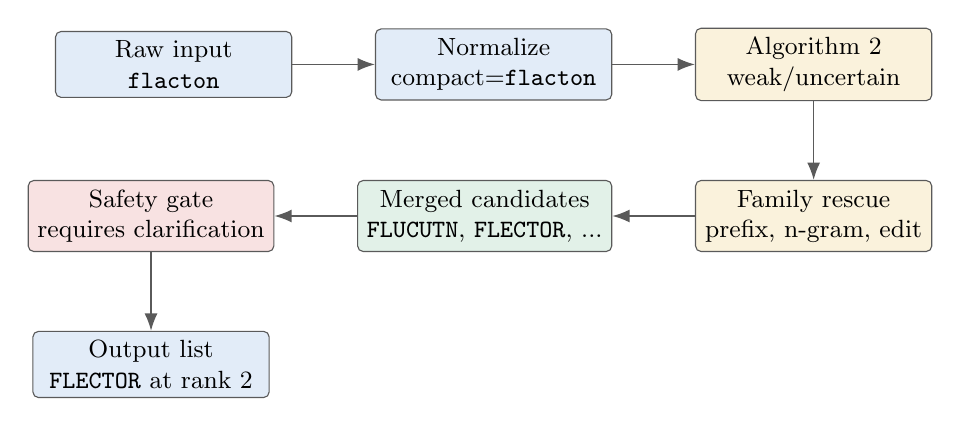
\begin{tikzpicture}[
  node distance=1.0cm and 1.05cm,
  box/.style={rectangle, rounded corners=2pt, draw=LineGray, align=center,
              minimum width=3.0cm, minimum height=0.82cm, font=\small},
  arrow/.style={-{Latex[length=2.2mm]}, draw=LineGray, line width=0.55pt}
]
\node[box, fill=BoxBlue] (q) {Raw input\\\id{flacton}};
\node[box, fill=BoxBlue, right=of q] (norm) {Normalize\\compact=\id{flacton}};
\node[box, fill=BoxYellow, right=of norm] (a2) {Algorithm 2\\weak/uncertain};
\node[box, fill=BoxYellow, below=of a2] (rescue) {Family rescue\\prefix, n-gram, edit};
\node[box, fill=BoxGreen, left=of rescue] (cands) {Merged candidates\\\id{FLU CUT N}, \id{FLECTOR}, ...};
\node[box, fill=BoxRed, left=of cands] (safe) {Safety gate\\requires clarification};
\node[box, fill=BoxBlue, below=of safe] (out) {Output list\\\id{FLECTOR} at rank 2};
\draw[arrow] (q) -- (norm);
\draw[arrow] (norm) -- (a2);
\draw[arrow] (a2) -- (rescue);
\draw[arrow] (rescue) -- (cands);
\draw[arrow] (cands) -- (safe);
\draw[arrow] (safe) -- (out);
\end{tikzpicture}%
}
\caption{Worked example flow. The rescue layer improves retrieval, and the
safety gate prevents an unsafe confident top-1.}
\end{figure}

\section{Root-Cause Lessons Learned}

\begin{table}[H]
\centering
\small
\begin{tabularx}{\linewidth}{L{0.23\linewidth}Y L{0.25\linewidth}}
\toprule
\textbf{Observed problem} & \textbf{Engineering lesson} & \textbf{Algorithm 4 action} \\
\midrule
Wrong answer is genuinely closer &
Some expected values are family-equivalence problems, not search problems. Example:
\id{levohista} is closer to \id{LEVOHISTAM} than \id{LEVOHISTAMIN}. &
Document acceptable-alternative / family-grouping work instead of forcing a farther string. \\
Equal edit distance tie &
Candidates can be equally close by edit distance, so the tiebreaker needs more evidence. &
Add same-position score, length coverage, first-character preference, and full-word fuzzy evidence. \\
Correct family missing from candidate pool &
Candidate generation was too narrow when the first letter was wrong. &
Try plausible first-letter variants and broaden the family rescue prefilter. \\
Prefix-only false positive &
A prefix or token fragment can look good while the full compact string is poor. &
Penalize weak partial-prefix matches when edit evidence is low. \\
Fuzzy recovery can be dangerous &
Finding a candidate is not the same as being safe to answer confidently. &
Keep clarification required for fuzzy/risky recovered candidates. \\
\bottomrule
\end{tabularx}
\caption{How the supplied mistakes were converted into general rules.}
\end{table}

\section{Benchmark Results}

\subsection*{Full V2 Results}

\begin{landscape}
\tiny
\setlength{\tabcolsep}{1.5pt}
\begin{longtable}{@{}L{0.065\linewidth}rL{0.10\linewidth}rL{0.09\linewidth}rrrrrrL{0.11\linewidth}L{0.13\linewidth}@{}}
\caption{Full V2 benchmark across every algorithm, with runtime and space columns added.}\\
\toprule
\textbf{Algorithm} & \textbf{Cases} & \textbf{Recorded runtime} & \textbf{ms/case} &
\textbf{Runtime note} & \textbf{Hit@1} & \textbf{Hit@20} & \textbf{Behavior} &
\textbf{Unsafe} & \textbf{No result} & \textbf{Avg pool} &
\textbf{Space meaning} & \textbf{Why this pool size happens} \\
\midrule
\endfirsthead
\toprule
\textbf{Algorithm} & \textbf{Cases} & \textbf{Recorded runtime} & \textbf{ms/case} &
\textbf{Runtime note} & \textbf{Hit@1} & \textbf{Hit@20} & \textbf{Behavior} &
\textbf{Unsafe} & \textbf{No result} & \textbf{Avg pool} &
\textbf{Space meaning} & \textbf{Why this pool size happens} \\
\midrule
\endhead
Algorithm 1 & 115,000 & A1+A2 joint: 152.44s & 1.33 &
Not isolated from Algorithm 2 in the recorded evaluator run. &
75.26\% & 88.40\% & 88.66\% & 0.02\% & 2.82\% & 188.85 &
Largest temporary candidate set. &
The current app evaluator keeps many product-row candidates before safety/ranking. \\
Algorithm 2 & 115,000 & A1+A2 joint: 152.44s & 1.33 &
Not isolated from Algorithm 1 in the recorded evaluator run. &
79.30\% & 91.84\% & 91.29\% & 6.40\% & 1.09\% & 17.86 &
Smallest temporary candidate set. &
The external fast algorithm is more aggressively indexed and usually returns a compact top candidate list. \\
Algorithm 3 & 115,000 & 161.88s & 1.41 &
Standalone master run. &
81.03\% & 93.09\% & 93.33\% & 0.00\% & 0.22\% & 37.69 &
Merged child candidate set. &
It runs Algorithm 1 and Algorithm 2, then merges duplicate commercial families and applies safety gates. \\
Algorithm 4 & 115,000 & 635.79s & 5.53 &
Standalone Algorithm 4 run after recommendation pass. &
81.86\% & 92.99\% & 93.09\% & 0.00\% & 0.92\% & 22.19 &
Bounded rescue candidate set. &
It keeps Algorithm 2 results, optionally adds context-clean results, then rescue-prefilters at most 40 families before returning top candidates. \\
\bottomrule
\end{longtable}
\setlength{\tabcolsep}{6pt}
\normalsize
\end{landscape}

\subsection*{Manual and Website Checks}

\begin{table}[H]
\centering
\small
\begin{tabular}{lrrrrrr}
\toprule
\textbf{Benchmark} & \textbf{Rows} & \textbf{Hit@1} & \textbf{Hit@20} & \textbf{Behavior} & \textbf{Unsafe} & \textbf{No result} \\
\midrule
Algorithm 4 manual failures & 50 & 58.00\% & 70.00\% & 70.00\% & 0.00\% & 0.00\% \\
Algorithm 4 proportional sample & 6,000 & 81.12\% & 92.83\% & 92.90\% & 0.00\% & 0.83\% \\
DrugEye trade sample & 6,000 & 21.75\% & 30.53\% & 30.53\% & 0.00\% & 62.88\% \\
\bottomrule
\end{tabular}
\caption{Additional checks run today. DrugEye is a public website baseline on
the same 6,000-row sample, not a full local-catalog algorithm.}
\end{table}

\begin{figure}[H]
\centering
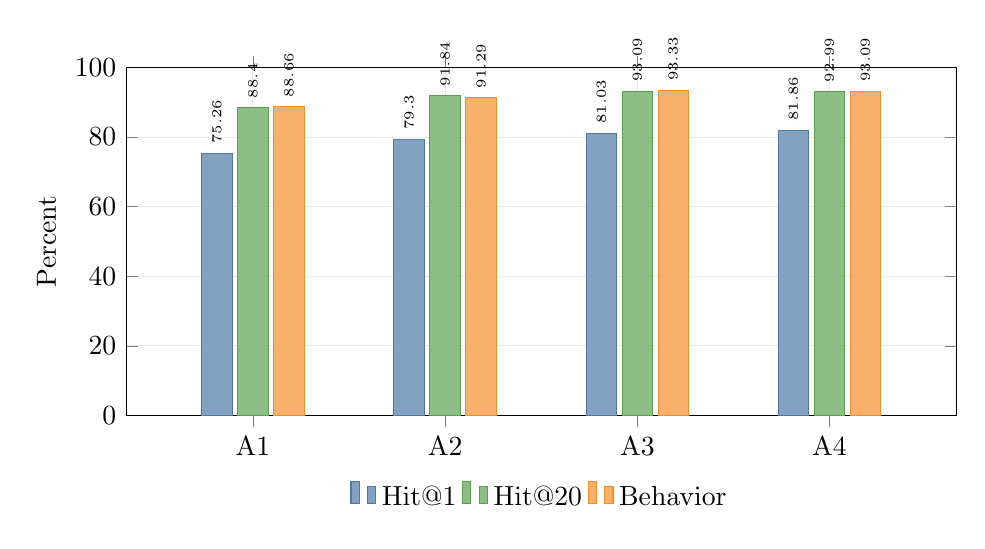
\begin{tikzpicture}
\begin{axis}[
    ybar,
    width=\linewidth,
    height=6.0cm,
    ymin=0,
    ymax=100,
    ylabel={Percent},
    symbolic x coords={A1,A2,A3,A4},
    xtick=data,
    bar width=11pt,
    enlarge x limits=0.22,
    legend style={at={(0.5,-0.17)}, anchor=north, legend columns=3, draw=none},
    nodes near coords,
    every node near coord/.append style={font=\tiny, rotate=90, anchor=west},
    grid=major,
    grid style={draw=gray!18}
]
\addplot[fill=BarBlue!70, draw=BarBlue] coordinates {
    (A1,75.26) (A2,79.30) (A3,81.03) (A4,81.86)
};
\addplot[fill=BarGreen!70, draw=BarGreen] coordinates {
    (A1,88.40) (A2,91.84) (A3,93.09) (A4,92.99)
};
\addplot[fill=BarOrange!70, draw=BarOrange] coordinates {
    (A1,88.66) (A2,91.29) (A3,93.33) (A4,93.09)
};
\legend{Hit@1, Hit@20, Behavior}
\end{axis}
\end{tikzpicture}
\caption{Full V2 quality comparison. The key tradeoff is Algorithm 4's higher
Hit@1 versus Algorithm 3's slightly stronger Hit@20 and behavior success.}
\end{figure}

\section{Time And Space Complexity}

Use these symbols:

\begin{table}[H]
\centering
\small
\begin{tabularx}{\linewidth}{L{0.14\linewidth}Y}
\toprule
\textbf{Symbol} & \textbf{Meaning} \\
\midrule
\(N\) & Product rows in the catalog. \\
\(F\) & Unique commercial families after grouping, \(F \leq N\). \\
\(L\) & Average compact commercial-name length. \\
\(Q\) & Compact query length. \\
\(C_1\) & Algorithm 1 candidate count for one query. \\
\(C_2\) & Algorithm 2 candidate count for one query. \\
\(C_r\) & Algorithm 4 rescue family candidates after bucket collection and prefiltering. \\
\(M\) & Algorithm 3 merged child candidates, usually bounded by child top-k results. \\
\(R\) & Algorithm 4 merged candidate count. \\
\bottomrule
\end{tabularx}
\caption{Complexity symbols.}
\end{table}

\begin{landscape}
\tiny
\setlength{\tabcolsep}{1pt}
\begin{longtable}{@{}L{0.07\linewidth}L{0.10\linewidth}L{0.13\linewidth}L{0.12\linewidth}L{0.11\linewidth}L{0.15\linewidth}L{0.15\linewidth}L{0.13\linewidth}@{}}
\caption{Detailed time, space, and quality analysis by algorithm.}\\
\toprule
\textbf{Algorithm} & \textbf{Observed full-run time} & \textbf{Quality scores} &
\textbf{Safety and failures} & \textbf{Observed query space} &
\textbf{Preprocessed space} & \textbf{Per-query work and memory} &
\textbf{Why the runtime/space looks like this} \\
\midrule
\endfirsthead
\toprule
\textbf{Algorithm} & \textbf{Observed full-run time} & \textbf{Quality scores} &
\textbf{Safety and failures} & \textbf{Observed query space} &
\textbf{Preprocessed space} & \textbf{Per-query work and memory} &
\textbf{Why the runtime/space looks like this} \\
\midrule
\endhead
Algorithm 1 &
A1+A2 joint evaluator: 152.44s for 115,000 rows, 1.33 ms/case. A1 was not isolated in that run. &
Hit@1 75.26\%; Hit@20 88.40\%; behavior 88.66\%. &
Behavior errors 13,045; no-result 2.82\%; unsafe confident top-1 0.02\%. &
Average candidate pool 188.85, the largest observed pool. &
\(\bigO(NL^2)\) worst-case index space from product rows, normalized keys, prefix/delete-key style lookup data, and safety metadata. &
\(\bigO(C_1QL + C_1\log C_1)\); keeps many product-row candidates while scoring and sorting. Temporary memory is approximately \(\bigO(C_1)\). &
Safer than Algorithm 2, but broad product-row recall means it carries far more candidates per query. \\
Algorithm 2 &
A1+A2 joint evaluator: 152.44s for 115,000 rows, 1.33 ms/case. A2 was not isolated in that run. &
Hit@1 79.30\%; Hit@20 91.84\%; behavior 91.29\%. &
Behavior errors 10,030; no-result 1.09\%; unsafe confident top-1 6.40\%. &
Average candidate pool 17.86, the smallest observed pool. &
\(\bigO(NL^2)\) worst-case index space plus typo features: n-grams, phonetic keys, skeleton keys, token statistics, and edit-distance support data. &
\(\bigO(Q^2 + C_2QL + C_2\log C_2)\); memory approximately \(\bigO(C_2)\). &
Fast and compact because it aggressively narrows candidates, but it is willing to be confidently wrong more often. \\
Algorithm 3 &
Standalone master run: 161.88s for 115,000 rows, 1.41 ms/case. &
Hit@1 81.03\%; Hit@20 93.09\%; behavior 93.33\%. &
Behavior errors 7,681; no-result 0.22\%; unsafe confident top-1 0.00\%. &
Average candidate pool 37.69 after merging child candidates. &
Algorithm 1 index space plus Algorithm 2 index space. It keeps both search stacks available. &
Algorithm 1 query + Algorithm 2 query + \(\bigO(M\log M)\) rank fusion; temporary memory is child query memory plus \(\bigO(M)\). &
More memory than Algorithm 2 because it merges two ranked lists, but stronger safety and behavior because Algorithm 1 can veto risky confidence. \\
Algorithm 4 &
Standalone Algorithm 4 run: 635.79s for 115,000 rows, 5.53 ms/case. &
Hit@1 81.86\%; Hit@20 92.99\%; behavior 93.09\%. &
Behavior errors 7,965; no-result 0.92\%; unsafe confident top-1 0.00\%. &
Average candidate pool 22.19. Smaller than Algorithm 3, larger than Algorithm 2. &
Algorithm 2 index space plus \(\bigO(FL^2)\) family rescue index over unique commercial families, not every product row. &
Algorithm 2 query + optional context-clean query + gated rescue. Rescue prefilter keeps at most 40 families for expensive scoring; output is top 20. Temporary memory is about \(\bigO(C_2 + C_r + R)\). &
It keeps fewer final candidates than Algorithm 3, but it does heavier rescue scoring per uncertain query, so the current Python run is slower. \\
\bottomrule
\end{longtable}
\setlength{\tabcolsep}{6pt}
\normalsize
\end{landscape}

\begin{figure}[H]
\centering
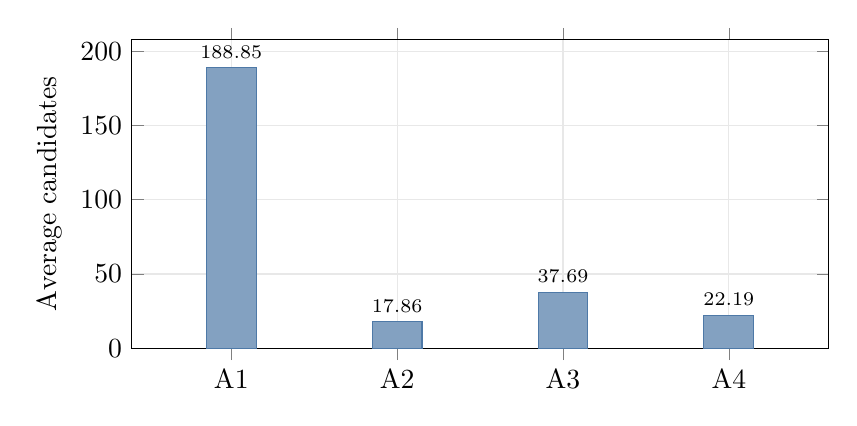
\begin{tikzpicture}
\begin{axis}[
    ybar,
    width=0.86\linewidth,
    height=5.5cm,
    ymin=0,
    ylabel={Average candidates},
    symbolic x coords={A1,A2,A3,A4},
    xtick=data,
    bar width=18pt,
    enlarge x limits=0.20,
    nodes near coords,
    every node near coord/.append style={font=\scriptsize},
    grid=major,
    grid style={draw=gray!18}
]
\addplot[fill=BarBlue!70, draw=BarBlue] coordinates {
    (A1,188.85) (A2,17.86) (A3,37.69) (A4,22.19)
};
\end{axis}
\end{tikzpicture}
\caption{Average candidate pool on full V2. Algorithm 4 keeps a smaller pool
than Algorithm 3, but its broader rescue logic made total runtime slower in the
current Python benchmark harness.}
\end{figure}

\section{Representative Test Cases}

\begin{table}[H]
\centering
\small
\begin{tabularx}{\linewidth}{L{0.24\linewidth}L{0.24\linewidth}Y}
\toprule
\textbf{Input} & \textbf{Expected output} & \textbf{What it exercises} \\
\midrule
\id{flacton} & \id{FLECTOR} & Manual failure recovered by Algorithm 4 at rank 2 after general rescue changes. \\
\id{Auticax} & \id{anticox} & Compound typo with edit-distance tie pressure; still fails and needs stronger general multi-error handling. \\
\id{levohista} & \id{levohistamin} & Shows acceptable-alternative risk because \id{LEVOHISTAM} is genuinely closer than expected. \\
\id{abc} & \id{__AMBIGUOUS__} or colliding family & Short prefix ambiguity; the safe behavior is clarification, not confidence. \\
\id{112} & \id{__NO_MATCH__} & Negative input that should not become a confident medicine match. \\
\id{aape renewal sunscreen spf 60ml} & \id{AAPE RENEWAL SUNSCREEN SPF} & Brand plus strength/form context; tests context cleanup. \\
\bottomrule
\end{tabularx}
\caption{Examples that explain the important behavior, not just the aggregate scores.}
\end{table}

\section{Category Error Table}

The table below compares all four algorithms on every V2 category. Hit@20 is the
retrieval score. Error count and error rate are based on behavior success, so
they include both retrieval misses and unsafe/wrong response-mode behavior.

\begin{landscape}
\tiny
\setlength{\tabcolsep}{1pt}
\begin{longtable}{@{}r L{0.045\linewidth} L{0.13\linewidth} r L{0.20\linewidth} r r r r r r r r r r r r@{}}
\caption{All-algorithm category-level scores, error counts, and error rates.}\\
\toprule
\textbf{\#} & \textbf{Scope} & \textbf{Category} & \textbf{Cases} & \textbf{Example} &
\textbf{A1 H@20} & \textbf{A2 H@20} & \textbf{A3 H@20} & \textbf{A4 H@20} &
\textbf{A1 Err} & \textbf{A2 Err} & \textbf{A3 Err} & \textbf{A4 Err} &
\textbf{A1 Err\%} & \textbf{A2 Err\%} & \textbf{A3 Err\%} & \textbf{A4 Err\%} \\
\midrule
\endfirsthead
\toprule
\textbf{\#} & \textbf{Scope} & \textbf{Category} & \textbf{Cases} & \textbf{Example} &
\textbf{A1 H@20} & \textbf{A2 H@20} & \textbf{A3 H@20} & \textbf{A4 H@20} &
\textbf{A1 Err} & \textbf{A2 Err} & \textbf{A3 Err} & \textbf{A4 Err} &
\textbf{A1 Err\%} & \textbf{A2 Err\%} & \textbf{A3 Err\%} & \textbf{A4 Err\%} \\
\midrule
\endhead
1 & \id{inside} & \id{single_letter_visual_confusion} & 8,000 & \id{edwinerve} $\rightarrow$ \id{ADWINERVE (visual_A_to_E_pos_0)} & 96.79\% & 99.71\% & 99.46\% & 99.76\% & 257 & 23 & 43 & 19 & 3.21\% & 0.29\% & 0.54\% & 0.24\% \\
2 & \id{inside} & \id{single_letter_phonetic_confusion} & 6,000 & \id{pabycare} $\rightarrow$ \id{BABY CARE (phonetic_B_to_P_pos_0)} & 99.58\% & 99.90\% & 99.90\% & 99.90\% & 25 & 6 & 6 & 6 & 0.42\% & 0.10\% & 0.10\% & 0.10\% \\
3 & \id{inside} & \id{multi_char_phonetic_confusion} & 5,000 & \id{sharcodoll} $\rightarrow$ \id{CHARCODOLL (multi_phonetic_ch_to_sh_pos_0)} & 97.70\% & 99.72\% & 99.66\% & 99.90\% & 115 & 14 & 17 & 5 & 2.30\% & 0.28\% & 0.34\% & 0.10\% \\
4 & \id{inside} & \id{ligature_confusion} & 4,000 & \id{dapom} $\rightarrow$ \id{ALAPOM (ligature_al_to_d_pos_0)} & 94.42\% & 97.32\% & 98.02\% & 99.33\% & 223 & 107 & 79 & 27 & 5.57\% & 2.68\% & 1.98\% & 0.68\% \\
5 & \id{inside} & \id{single_char_deletion_position_weighted} & 5,000 & \id{3candyadults} $\rightarrow$ \id{D3 CANDY ADULTS (deletion_first_char_pos_0)} & 95.72\% & 99.88\% & 99.76\% & 99.92\% & 214 & 6 & 12 & 4 & 4.28\% & 0.12\% & 0.24\% & 0.08\% \\
6 & \id{inside} & \id{single_char_insertion} & 3,000 & \id{asafetriumkids} $\rightarrow$ \id{SAFETRIUM KIDS (insertion_adjacent_key_letter_at_pos_0)} & 98.87\% & 99.97\% & 99.73\% & 99.97\% & 34 & 1 & 8 & 1 & 1.13\% & 0.03\% & 0.27\% & 0.03\% \\
7 & \id{inside} & \id{transposition_position_weighted} & 3,000 & \id{abrmon} $\rightarrow$ \id{BARMON (transposition_early_pos_0)} & 98.43\% & 99.83\% & 99.73\% & 99.83\% & 47 & 5 & 8 & 5 & 1.57\% & 0.17\% & 0.27\% & 0.17\% \\
8 & \id{inside} & \id{truncation_doctor_abbreviation} & 6,000 & \id{abc} $\rightarrow$ \id{ABC IMMUNE (truncation_prefix_len_3)} & 80.83\% & 83.67\% & 85.92\% & 64.15\% & 1,150 & 980 & 845 & 2,151 & 19.17\% & 16.33\% & 14.08\% & 35.85\% \\
9 & \id{inside} & \id{two_error_combinations} & 8,000 & \id{abgentp} $\rightarrow$ \id{APIGENT P (deletion_plus_phonetic_variant_0)} & 84.09\% & 93.77\% & 94.05\% & 98.16\% & 1,273 & 498 & 476 & 147 & 15.91\% & 6.23\% & 5.95\% & 1.84\% \\
10 & \id{inside} & \id{three_error_combinations} & 5,000 & \id{acalagnhair} $\rightarrow$ \id{SCALOGEN HAIR (keyboard_vowel_delete_variant_0)} & 54.08\% & 75.42\% & 77.36\% & 90.64\% & 2,296 & 1,229 & 1,132 & 468 & 45.92\% & 24.58\% & 22.64\% & 9.36\% \\
11 & \id{inside} & \id{speed_typing_errors} & 3,000 & \id{aabilifymaintena} $\rightarrow$ \id{ABILIFY MAINTENA (double_first_letter)} & 89.97\% & 99.73\% & 99.67\% & 99.77\% & 301 & 8 & 10 & 7 & 10.03\% & 0.27\% & 0.33\% & 0.23\% \\
12 & \id{inside} & \id{wrong_vowels_in_consonant_frame} & 5,000 & \id{aasyiron} $\rightarrow$ \id{EASY IRON (wrong_1_vowels_variant_0)} & 98.36\% & 98.78\% & 98.76\% & 99.22\% & 82 & 61 & 62 & 39 & 1.64\% & 1.22\% & 1.24\% & 0.78\% \\
13 & \id{inside} & \id{punctuation_whitespace_copy_paste_artifacts} & 1,000 & \id{2hc t} $\rightarrow$ \id{2HC T (copy_paste_artifact_0)} & 100.00\% & 100.00\% & 100.00\% & 100.00\% & 0 & 0 & 0 & 0 & 0.00\% & 0.00\% & 0.00\% & 0.00\% \\
14 & \id{inside} & \id{case_sensitivity} & 500 & \id{2hC t} $\rightarrow$ \id{2HC T (case_alternating_case)} & 100.00\% & 100.00\% & 100.00\% & 100.00\% & 0 & 0 & 0 & 0 & 0.00\% & 0.00\% & 0.00\% & 0.00\% \\
15 & \id{inside} & \id{number_word_confusion} & 500 & \id{ALICO VITAMIN DTHREE} $\rightarrow$ \id{ALICO VITAMIN D3 (number_word_variant_0)} & 97.20\% & 98.20\% & 98.40\% & 98.40\% & 14 & 9 & 8 & 8 & 2.80\% & 1.80\% & 1.60\% & 1.60\% \\
16 & \id{semi_outside} & \id{embedded_form_strength_parsing} & 4,000 & \id{aape renewal sunscreen spf 60ml} $\rightarrow$ \id{AAPE RENEWAL SUNSCREEN SPF (brand_strength)} & 96.97\% & 87.70\% & 97.32\% & 99.40\% & 121 & 493 & 107 & 24 & 3.02\% & 12.32\% & 2.68\% & 0.60\% \\
17 & \id{safety} & \id{dangerous_ed1_pairs} & 5,000 & \id{aba} $\rightarrow$ \id{ALBA (dangerous_ed1_deletion_variant_0)} & 83.86\% & 96.68\% & 94.48\% & 97.52\% & 807 & 166 & 276 & 124 & 16.14\% & 3.32\% & 5.52\% & 2.48\% \\
18 & \id{safety} & \id{substring_traps} & 3,000 & \id{abimol} $\rightarrow$ \id{ABIMOL EXTRA (substring_long_truncated_to_short)} & 77.97\% & 79.40\% & 82.13\% & 78.93\% & 661 & 618 & 536 & 632 & 21.41\% & 20.60\% & 17.87\% & 21.07\% \\
19 & \id{safety} & \id{negative_no_match_expected} & 3,000 & \id{112} $\rightarrow$ \id{__NO_MATCH__ (negative_catalog_metadata)} & 99.97\% & 99.83\% & 100.00\% & 100.00\% & 1 & 5 & 0 & 0 & 0.03\% & 0.17\% & 0.00\% & 0.00\% \\
20 & \id{safety} & \id{contradictory_form_route} & 2,000 & \id{acetylcysteine vita ear drops} $\rightarrow$ \id{ACETYLCYSTEINE VITA (contradictory_form_ear_drops)} & 99.95\% & 99.95\% & 99.95\% & 99.90\% & 1 & 1 & 1 & 2 & 0.05\% & 0.05\% & 0.05\% & 0.10\% \\
21 & \id{safety} & \id{cancelled_na_drug_lookup} & 1,000 & \id{acnesol} $\rightarrow$ \id{ACNESOL (cancelled_exact)} & 99.40\% & 99.80\% & 99.70\% & 99.70\% & 6 & 2 & 3 & 3 & 0.60\% & 0.20\% & 0.30\% & 0.30\% \\
22 & \id{safety} & \id{score_gap_ambiguity_detection} & 4,000 & \id{act} $\rightarrow$ \id{__AMBIGUOUS__ (score_gap_ed1_collision_proxy)} & 91.27\% & 86.05\% & 91.90\% & 84.47\% & 63 & 1,000 & 63 & 546 & 1.58\% & 25.00\% & 1.58\% & 13.65\% \\
23 & \id{inside} & \id{ocr_letter_digit_confusion} & 4,000 & \id{99q9999999rr} $\rightarrow$ \id{9999999999RR (ocr_9_to_Q_pos_2)} & 98.98\% & 99.85\% & 99.92\% & 99.85\% & 41 & 6 & 3 & 6 & 1.02\% & 0.15\% & 0.08\% & 0.15\% \\
24 & \id{inside} & \id{ocr_plus_other_error_combined} & 3,000 & \id{0ctomtol} $\rightarrow$ \id{OCTOMOTOL (ocr_plus_deletion_pos_0)} & 92.07\% & 94.27\% & 95.97\% & 98.60\% & 238 & 172 & 121 & 42 & 7.93\% & 5.73\% & 4.03\% & 1.40\% \\
25 & \id{inside} & \id{double_letter_reduction_expansion} & 3,000 & \id{bbactroban} $\rightarrow$ \id{BACTROBAN (double_expansion_B_to_BB_pos_0)} & 99.87\% & 99.93\% & 99.90\% & 99.93\% & 4 & 2 & 3 & 2 & 0.13\% & 0.07\% & 0.10\% & 0.07\% \\
26 & \id{inside} & \id{keyboard_adjacent_sampled} & 2,000 & \id{qbcimmune} $\rightarrow$ \id{ABC IMMUNE (keyboard_adjacent_A_to_Q_sampled_pos_0)} & 91.00\% & 98.80\% & 97.50\% & 98.80\% & 180 & 24 & 50 & 24 & 9.00\% & 1.20\% & 2.50\% & 1.20\% \\
27 & \id{inside} & \id{four_plus_error_combinations} & 4,000 & \id{abksunblck} $\rightarrow$ \id{APIC SUN BLOCK (ligature_two_phonetic_delete_variant_0)} & 50.82\% & 69.42\% & 72.78\% & 85.78\% & 1,967 & 1,223 & 1,089 & 569 & 49.18\% & 30.57\% & 27.22\% & 14.22\% \\
28 & \id{inside} & \id{consonant_frame_wrong_vowels_heavy} & 4,000 & \id{2mwhytisbyagimyren} $\rightarrow$ \id{2M WHITES BEEGU MARIN (all_vowels_wrong)} & 97.08\% & 97.95\% & 98.00\% & 98.83\% & 117 & 82 & 80 & 47 & 5.53\% & 2.05\% & 2.00\% & 1.18\% \\
29 & \id{inside} & \id{multi_word_name_fragmentation} & 2,000 & \id{cal d} $\rightarrow$ \id{CALNESIA D (abbreviated_tokens)} & 62.20\% & 70.80\% & 68.80\% & 69.75\% & 756 & 584 & 624 & 605 & 37.80\% & 29.20\% & 31.20\% & 30.25\% \\
30 & \id{inside} & \id{autocorrect_artifacts} & 2,000 & \id{foster} $\rightarrow$ \id{FASTER (autocorrect_vowel_correction)} & 1.85\% & 3.60\% & 3.45\% & 3.50\% & 1,963 & 1,928 & 1,931 & 1,930 & 98.15\% & 96.40\% & 96.55\% & 96.50\% \\
31 & \id{smoke} & \id{exact_match_baseline} & 2,000 & \id{2HC T} $\rightarrow$ \id{2HC T (exact_base_group)} & 100.00\% & 100.00\% & 100.00\% & 100.00\% & 0 & 0 & 0 & 0 & 0.00\% & 0.00\% & 0.00\% & 0.00\% \\
32 & \id{smoke} & \id{exact_match_with_strength} & 2,000 & \id{ABC MOCOTIVE 70ML} $\rightarrow$ \id{ABC MOCOTIVE (exact_brand_with_real_strength)} & 100.00\% & 95.85\% & 100.00\% & 98.55\% & 0 & 83 & 0 & 29 & 0.00\% & 4.15\% & 0.00\% & 1.45\% \\
33 & \id{smoke} & \id{keyboard_shift_whole_word} & 500 & \id{aahaxis} $\rightarrow$ \id{SAJA COD (keyboard_shift_left)} & 82.40\% & 0.40\% & 82.40\% & 1.40\% & 88 & 498 & 88 & 493 & 17.60\% & 99.60\% & 17.60\% & 98.60\% \\
34 & \id{smoke} & \id{prefix_ambiguity_awareness} & 1,500 & \id{ace} $\rightarrow$ \id{__AMBIGUOUS__ (ambiguous_prefix_len_3)} & 99.40\% & 99.73\% & 99.73\% & 97.67\% & 0 & 196 & 0 & 0 & 0.00\% & 13.07\% & 0.00\% & 0.00\% \\
\bottomrule
\end{longtable}
\setlength{\tabcolsep}{6pt}
\normalsize
\end{landscape}

\begin{figure}[H]
\centering
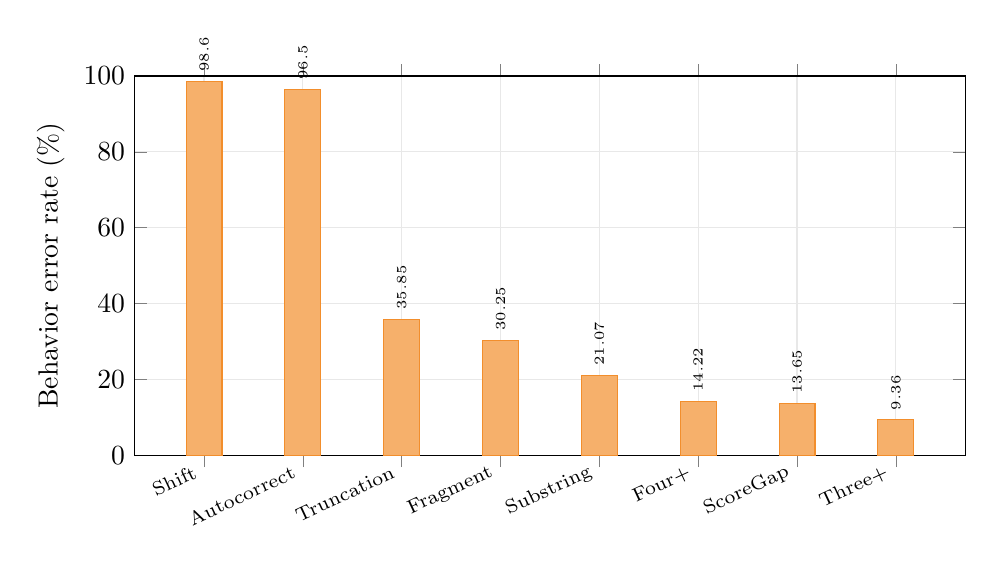
\begin{tikzpicture}
\begin{axis}[
    ybar,
    width=\linewidth,
    height=6.4cm,
    ymin=0,
    ymax=100,
    ylabel={Behavior error rate (\%)},
    symbolic x coords={Shift,Autocorrect,Truncation,Fragment,Substring,Four+,ScoreGap,Three+},
    xtick=data,
    x tick label style={rotate=25, anchor=east, font=\scriptsize},
    bar width=13pt,
    enlarge x limits=0.10,
    nodes near coords,
    every node near coord/.append style={font=\tiny, rotate=90, anchor=west},
    grid=major,
    grid style={draw=gray!18}
]
\addplot[fill=BarOrange!70, draw=BarOrange] coordinates {
    (Shift,98.60)
    (Autocorrect,96.50)
    (Truncation,35.85)
    (Fragment,30.25)
    (Substring,21.07)
    (Four+,14.22)
    (ScoreGap,13.65)
    (Three+,9.36)
};
\end{axis}
\end{tikzpicture}
\caption{Highest Algorithm 4 behavior-error rates by category. The biggest
remaining failures are whole-keyboard shifts, autocorrect artifacts, short
truncations, and fragmented multi-word names.}
\end{figure}

\section{Engineering Takeaways}

\begin{itemize}
  \item The most important correction was ethical and methodological: do not
        memorize the manual failures. The benchmark is only useful if the code
        learns general patterns.
  \item Algorithm 4 now learns from failure categories, not individual answers.
        The added rules are first-letter variants, tie-breaking evidence,
        partial-prefix penalties, and broader confusion groups.
  \item Algorithm 4 improves full Hit@1 over Algorithm 3, but Algorithm 3 still
        wins on Hit@20 and behavior success. That makes Algorithm 3 the safer
        current baseline.
  \item DrugEye performs much worse on the V2 sample, mostly because many noisy
        generated inputs produce no website result.
  \item The hardest remaining categories are not ordinary typos. They are
        whole-keyboard shifts, autocorrect artifacts, short truncations,
        fragmented multi-word names, substring traps, and score-gap ambiguity.
  \item Next work should focus on family-equivalence labels, acceptable
        alternatives, better multi-token compact matching, and a separate
        whole-keyboard-shift decoder.
\end{itemize}

\end{document}
